%!TEX root = ../thesis.tex
\documentclass[..thesis.tex]{subfiles}
\hyphenation{re-gis-tering}
\begin{document}
\subsection{Overview}

\kalmer{See ülevaade ei anna lugejale mitte midagi --- selle võid lihtsalt ära jätta.}
\todisc{Mulle tundub liiga karm otse liidesest alustada, jätaks selle osa ikkagi sisse. Ei ole päris põhimõtteline,  kui Vesal arvab ka, et võiks maha võtta, siis võtame maha.}


To explain the role of device drivers, let's introduce two common devices that are usable on computers running a Linux operating system.

First of them is \inlinecode{/dev/tty}, a device that represents the terminal controlling the current process \cite{torvalds_linux}.
Opening a terminal in Linux and writing to the device results in the text being displayed in the terminal. One can try this with the following command: 

\inlinecode{echo "Hello" > /dev/tty}.
 
The second device we will introduce is \inlinecode{/dev/null}, a device that discards any data sent to it. So, redirecting text to this device has no effect.
One can send text to the device as follows:

\inlinecode{echo "Hello" > /dev/null}.

Although the two devices act differently, they can be both used in the same way -- we can redirect text to them (and redirect text from them).
This allows us to group the two devices together when reasoning about how to use them. The benefits of this are far greater when the number of devices that can be grouped together grows.

The role of Linux device drivers is to enable such groupings that can contain an arbitrary amount of devices.

This is done by enabling access to the devices via a small set of well-defined interfaces that other parts of the Linux kernel can make use of. 

In this paper, we will focus on a subset of device drivers called \textit{character (char) device drivers}.
Character device drivers allow unbuffered access to the underlying ``hardware''. Both of the drivers for the example devices above are char drivers.

\subsection{Interface of a character device driver}

Devices are exposed to the end user as entries in the file system and therefore it is natural
to use the same terminology for talking about device drivers' operations as about normal file operations.
Device drivers expose endpoints for \textit{reading}, \textit{writing to}, \textit{opening} and \textit{releasing} devices.
This list is not exhaustive\cite[include/linux/fs.h]{torvalds_linux}, but it is not necessary for a driver to expose them all.

As a running example we will introduce the driver \inlinecode{Counter}.
Counter keeps track of the difference between how many times the kernel has read from it and how many times the kernel has written to it
\footnote{The full source code is available in Appendix \ref{A:example-driver}}.

In the following code snippet, the parameters of the functions are omitted as they are not relevant for this example.



\begin{lstlisting}[language=C,style=def]
static ssize_t file_read(...){
    ++i;
    printk("Increasing i, new value:: %d \n",i);
    ...
}

static ssize_t file_write(...){
    --i;
    printk("Decreasing i, new value: %d \n",i);
    ...
}

static int file_open(...)
{
    printk("Opening device \n");
    return 0;
}

static int file_release(...){
    printk("Closing device \n");
    return 0;
}


\end{lstlisting}

The \inlinecode{read} function increases the global counter by one, while the \inlinecode{write} function decreases it by one.
Both the \inlinecode{open} and \inlinecode{release} functions only output info to the kernel log.

When the user reads from a file that exposes the driver, one can see that the file was opened, read and then closed. For a concrete example,
\inlinecode{head -c 1 < counter} produces the following entries in the kernel log:

\begin{lstlisting}[language=sh,style=def]
vootele kernel: Opening file 
vootele kernel: Increasing i, new value: 1 
vootele kernel: Closing file 
\end{lstlisting}

And similarly, when writing to the file, for example with \inlinecode{echo hi > my-driver}, the file is opened, written into and then closed.


Drivers expose devices to the kernel via \inlinecode{file operations} structure. When registering a driver to the kernel,
the file operations structure is registered with the kernel, which can invoke any of the methods specified in the structure.

The file operations structure of Counter is 

\begin{lstlisting}[language=c,style=def]
static struct file_operations f_ops = {
  .write   = file_write,
  .read    = file_read,
  .open    = file_open,
  .release = file_close,
};
\end{lstlisting}

Device drivers also expose \inlinecode{init} and \inlinecode{exit}, which the kernel can use to register and de-register a device driver. In case of Counter,
registering the device initializes the counter \inlinecode{i} to zero and then registers the file operations. 

\subsection{Data races in device drivers}

When registering our driver, we exposed multiple endpoints to the kernel. From that moment onwards, kernel can invoke any of the registered methods,
at any time, until the driver is de-registered. 

\toguide{ Why are data-races relevant for Linux device drivers?}

The multitude of entry points to the programs and lack of control over when they are entered makes avoiding \textit{data races} a challenge when writing Linux device drivers.
We say that data race occurs in a program when different threads simultaneously attempt to access a shared memory location and at least one of the accesses is a
write operation.

For an example of a data race in device drivers, it is quite obvious that when one writes to a device exposed by the example driver concurrently,
then the value of the counter after all the write operations is not determined -- it is easily possible that between the read and write operations of the counter, its value gets updated.

To be more concrete, in Figure \ref{fig:driver-race} is a snippet of the kernel log after running a script \footnote{Available in Appendix \ref{A:test-script}}
that reads and writes to the example driver in a loop that runs 10 000 times in 3 processes at the same time.
As the read operation increases $i$ and the write operation decreases it, the expected value without a data race would have been $0$.


\begin{figure}[H]
\centering
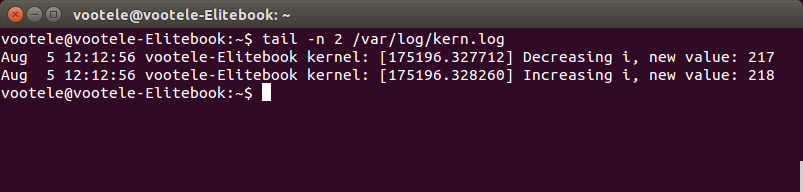
\includegraphics[width=0.9\textwidth]{driver-race}
\caption{Snippet from the kernel log after data race in an example device driver.}
\label{fig:driver-race}
\end{figure}


\toguide{ There are ways around them, right?}

To avoid data races, Linux kernel offers multiple locking primitives. 

A popular locking primitive is the \textit{spinlock}, which runs a tight loop, inside which it tries to acquire the lock until it succeeds.
This tight loop gives the lock its name. Using spinlocks avoids explicitly putting the thread to sleep when acquiring a lock fails.
If it is known that lock is held only for a very short time then the computational cost of putting a thread to sleep and then later awakening
it out-weights the extra CPU cycles used by the tight loop of a spinlock.

Spinlocks also offer a lock that differentiates between reads and writes, allowing multiple concurrent reads.

One of the most commonly used locking primitives is the \textit{mutually exclusive lock} (mutex). It also the one that should be used, if possible
\cite[Documentation/locking/mutex-design.txt]{torvalds_linux}. Older implementations of mutex put the thread to sleep if acquiring the lock failed,
whereas the current implementation is also capable of spinning for a limited time before resorting to explicitly putting the thread to sleep.

To eliminate a possible data race from our example driver, we could add a lock to the driver and acquire it on every read and write operation.
With the added lock, the read operation would look as follows:

\begin{lstlisting}[language=C,style=def]
static ssize_t file_read(...){
    mutex_lock(&my_mutex);
    ++i;
    printk("Increasing i, new value: %d \n",i);
    mutex_unlock(&my_mutex);
    ...
}
\end{lstlisting}

where \inlinecode{my\_mutex} is a static mutex.

After adding the same locking pattern to write operations, data race will no longer plague the example driver.

\subsection{Impact of data races on device drivers}

We have seen that data races are a real possibility in device drivers and also that there are ways to protect oneself against them. 

\toguide{ Why are the data-races prevalent?}

As previously discussed, Linux device drivers usually have multiple entry points and no control over when they are entered. Also, the device drivers are written in C,
a low level language, that makes reasoning about them quite challenging. Furthermore, quite often the person writing a driver is an expert on the device that the driver is for,
and not so much an expert on the Linux device drivers themselves. This makes correct usage of constructs that help to avoid data races difficult and error-prone.

\toguide{ How common are the data races?}

\kalmer{selle võiksid tõsta sissejuhatusse --- muu agiteerimise ja reklaami sisse}
\todisc{Minu arvates oluline siin sügavamalt üle käia, see aitas mul endal aru saada, et see on on probleem, mille lahendamiseks võib vaeva näha küll.}

Empirical studies validate this assertion. In a study done by Chou \textit{et al}. \cite{chou_empirical_2001} it was found that error rates in device drivers are three to seven times higher than in rest of the kernel. 

The situation seems to have become better over time. In the follow-up study conducted by Palix \textit{et al.} \cite{palix_faults_2011}, the error rate in device drivers improved, but drivers still contained the highest number of errors.

In a study done by Ryzhyk and others \cite{ryzhyk_dingo_2009}, out of the 498 bugs found between 2002 and 2008 in 13 selected Linux device drivers, 93 were concurrency related -- mainly data races or deadlocks. 

Mutilin \textit{et al.} \cite{mutilin_analysis_2012} found that data races are the most common single type of bug, remarkable 5 times more common than deadlocks in the Linux device drivers.

It is worth noting that based on \cite{chou_empirical_2001,palix_faults_2011}, the average lifetime of a bug is 18 months, making it quite likely that the bug makes its way to a stable version. 

\toguide{ How bad are they?}

In addition to being common, the bugs in device drivers can cause crashes fatal to the whole system. In Windows XP, 85\% of the reported failures were caused by issues with the device drivers \cite{swift_improving_2003}.

The data races are extremely unpleasant in safety-critical applications, where their presence could endanger lives. For that reason, the verification requirements of device drivers in safety-critical domains (for example aviation or automobile industry) are very rigorous, making the testing process very costly and time-consuming.

\end{document}
